\documentclass{webofc}
\usepackage[varg]{txfonts}   

\usepackage{graphicx}

\usepackage{todonotes}
\usepackage[capitalise,nameinlink]{cleveref}
%Nice formats for \cref
\crefname{section}{Sect.}{Sect.}
\Crefname{section}{Section}{Sections}
\crefname{listing}{\lstlistingname}{\lstlistingname}
\Crefname{listing}{Listing}{Listings}
\usepackage{pgfplots}

% Use package for subfigures
\usepackage{subcaption}

% layout changes
\setlength\belowcaptionskip{-15pt}
\renewcommand*{\bibfont}{\footnotesize}


\begin{document}
\title{Modeling and Simulation of Load Balancing Strategies for Computing in High Energy Physics}

\author{
	\firstname{Ren\'e} \lastname{Caspart}\inst{1}\fnsep\thanks{\email{rene.caspart@cern.ch}} \and
	\firstname{Patrick} \lastname{Firnkes}\inst{2}\fnsep\thanks{\email{patrick.firnkes@student.kit.edu}} \and
	\firstname{Manuel} \lastname{Giffels}\inst{1}\fnsep\thanks{\email{manuel.giffels@cern.ch}} \and
	\firstname{Anne} \lastname{Koziolek}\inst{2}\fnsep\thanks{\email{koziolek@kit.edu}} \and
	\firstname{G\"unter} \lastname{Quast}\inst{1}\fnsep\thanks{\email{g.quast@kit.edu}} \and
	\firstname{Ralf} \lastname{Reussner}\inst{2}\fnsep\thanks{\email{reussner@kit.edu}} \and
	\firstname{Maximilian} \lastname{Stemmer-Grabow}\fnsep\thanks{\email{mail@mxsg.de}}\inst{2}
}

\institute{
	Institute for Experimental Particle Physics (ETP) 
	\and
   Institute for Program Structures and Data Organization (IPD) \\
	at Karlsruhe Institute of Technology (KIT), Karlsruhe, Germany
}


\abstract{%
	The amount of data to be processed by experiments in high energy physics (HEP) is tremendously increasing in the coming years. To cope with this increasing load, most efficient usage of the resources is mandatory. Furthermore, the computing resources for user jobs in HEP will be increasingly distributed and heterogeneous, resulting in more difficult scheduling due to the increasing complexity of the system.
	We aim to create a simulation for the WLCG helping the HEP community to solve both challenges: a more efficient utilization of the grid and coping with the rising complexity of the system.
	There is currently no simulation existing helping the operators of the grid to make the correct decisions while optimizing the load balancing strategy.
	
	This paper presents a proof of concept in which the computing jobs at the Tier 1 center GridKa are modeled and simulated. To model the computing jobs we extended the Palladio simulator with a mechanism to simulate load balancing strategies. Furthermore, we implemented an automated model parameter analysis and model creation.
	
	Finally, the simulation results are validated using real word performance data. Our results suggest that simulating larger parts of the grid is feasible and can help to optimize the utilization of the grid.
}%
\maketitle
%

\section{Introduction}
\label{sec:intro}

The amount of data processed by experiments in high energy physics (HEP) will drastically increase in the coming years due the upgrade of the LHC to the High-Luminosity Large Hadron Collider (HL-LHC), creating major challenges for the HEP community \cite{community}.
\Cref{resources} shows the estimated required and provided CPU resources for the ATLAS experiment in the next ten years. Assuming a flat computing budget model, the estimated provided resources do not cover future needs for computing resource in the period from 2026 to 2028 due the start of the HL-LHC era. One of the key aspects to deal with this increasing load is the more efficient usage of existing resources.

Another challenge for the HEP community is the increasing heterogeneity and distribution of the computing resources of user jobs. Cloud resources, such as HNSciCloud and AWS, or institute clusters and Tier 3 centers will be progressively introduced for the computation of these jobs. This results in a more complex scheduling, because each resource has different optimal job types and mixes. Furthermore, this leads to a more dynamic data placement, where fewer centers host data and thus remote access is increasing.

\begin{figure*}
	\centering
	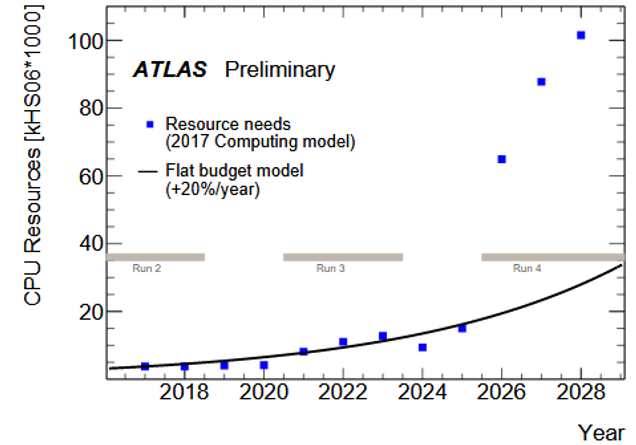
\includegraphics[width=0.5\linewidth]{images/resources}
	\caption[]{Estimated CPU resources of ATLAS \cite{community}}
	\label{resources}
\end{figure*}

We aim to create a simulation for the WLCG helping the HEP community to solve both challenges: a more efficient utilization of the grid and coping with the rising complexity of the system.
Currently, there is no model or simulation in existence to evaluate the load balancing strategies of the grid, helping the operators to make the correct decisions while optimizing the load balancing strategy.
\Cref{related} describes different attempts to simulate the WLCG or parts of it. However, they showed scalability issues or the simulations do not have the necessary detail level to simulate effects on working nodes that is necessary to evaluate load balancing strategies.

Optimizing load balancing strategies without the help of simulations requires stable load, in order to preserve the comparability of the different strategies. This is neither possible to achieve for the WLCG nor for a single center like GridKa, because the nature of the load is highly dynamical. Another option would be to use an isolated test system for the evaluation. However, the system under inspection is too large and thus a similar test systems would not be financially affordable. A smaller test system could not deliver correct results because too much of the complexity of the system would be taken away.
These reasons lead to the conclusion that a model and simulation of the performance of computing jobs is required to evaluate different load balancing strategies.

Our long term goal is to evaluate different load balancing strategies for the WLCG and additionally evaluate different design decisions affecting the performance of the grid. These gained insights will help the HEP community to solve the challenges caused by the HL-LHC upgrade.

The contribution of this paper is the modeling and simulating of CMS computing jobs at the Tier 1 center GridKa as a proof of concept.
The model and simulation are created using the Palladio simulator, see \Cref{sec:palladio} for details on Palladio. We chose Palladio to achieve a scalable simulation because it is a comparably abstract simulator (\Cref{related} gives an overview on other simulators and approaches).
This leads to the research question how we can use Palladio to evaluate load balancing strategies for the CMS computing jobs, because the simulation of load balancing strategies is a new use case for Palladio. To realise it we created an extension for the simulator that enables us to simulate load balancing strategies and furthermore, we created an automated model parameter analysis and model creation, in order to increase the usability of the simulation.
This model makes it possible to evaluate different load balancing strategies for GridKa and enables us to draw conclusions about the best optimizations of the load balancing for the WLCG. Also, it can be used as a foundation for models and simulations of larger parts of the WLCG.


This paper is organized as follows: \Cref{sec:palladio} presents the Palladio simulator as a foundation of the simulation. \Cref{sec:process} gives a overview on the simulation process. \Cref{sec:model} describes how different elements of the computing jobs and the computing resources are represented in our model. \Cref{sec:param} explains how we determine the model parameters and the automated model creation works. The validation is presented in \Cref{validation} and \Cref{related} puts our work in context with the related work. In \Cref{outlook} possible design decisions and how they could be modeled and simulated are presented. Finally, \Cref{conlusion} gives a conclusion on this paper.


\section{Foundations: Palladio}
\label{sec:palladio}
Palladio is a model driven software architecture simulator, which is implemented as an eclipse plugin and developed by Karlsruhe Institute of Technology (KIT), FZI Research Center for Information Technology, and University of Paderborn. Palladio predicts quality of software properties (e.g. performance) using several models of a system \cite{BECKER20093}.

These models are the component model, the assembly model, the resource model, the allocation model, and the usage model.
\begin{itemize}
	\item The component model: Specifies the structure and behavior of the components independently from their later usage. This allows reuse of the components, but requires its parametrization.
	\item The assembly model: Represents how the components are connected to model the software architecture.
	\item The resource model: Describes the resource environment. It contains the number and characteristics of the resource containers on which the components could be deployed and the topology of the network connecting these containers.
	\item The allocation model: Represents the mapping of the different components to the resource containers.
	\item The usage model: Defines the usage of a system regarding workload, user behavior, and parameters.
	
\end{itemize}
Once these models are created, Palladio can be used to simulate the system choosing one of several supported simulators. 

Lehrig and Becker \cite{arch} extended Palladio with Architectural Templates to make it possible to model cloud computing environments efficiently.
Furthermore, Palladio's simulation approach SimuLizar was created to simulate self-adaptive systems \cite{becker2013simulizar}.
It was later extended to support the metrics scalability, elasticity, and efficiency.

Palladio has been successfully used to solve several industrial problems and was used to optimize cloud infrastructure in the context of chemical computing as part of the CACTOS project \cite{rapidtesting}. 

\section{Simulation Process}
\label{sec:process}
To receive a valid model of a site and its jobs, we created the simulation process depicted in \Cref{process}. This process consists of five phases: Matching of data sets, grouping the data for job types, analysing the model parameters, generating a blueprint model, and lastly injecting the parameters into this model. Note, only a part of the data is used to calibrate the model, the other part is used for its validation.

The starting point of the simulation process is matching the data sets from different data sources as a prerequisite  of the analysis. In our proof of concept we have three data sources: The CERN WMArchive, CMS GridKa job data and GridKa node performance data. These data sets have to be matched because each set contains different information about an executed job, but none of them contains the complete information about it.

After matching and grouping the data for job types, the analysis of the job and working node data to extract performance parameters for the model takes place. For example, these are the CPU demand of jobs, the frequency of the job types or the CPU power of the nodes. This analysis and the data set matching are automated and described in \Cref{sec:param}.

The next step is the generation of the model of GridKa and the injection of the previously extracted performance parameters. Both steps do not require manually modeling. At this point the users have a valid and calibrated model of GridKa with its resource and the workload. The properties of this model are described in \Cref{sec:model}.

Users can then either run the simulation or make changes to the model to simulate the effect of a design change. 
Finally, after running the simulation, they can inspect the results, such as core utilization of a node or throughput of jobs, using the integrated visualization tool or they can export the results and use a third party software to do the evaluation.

\begin{figure*}
	\centering
	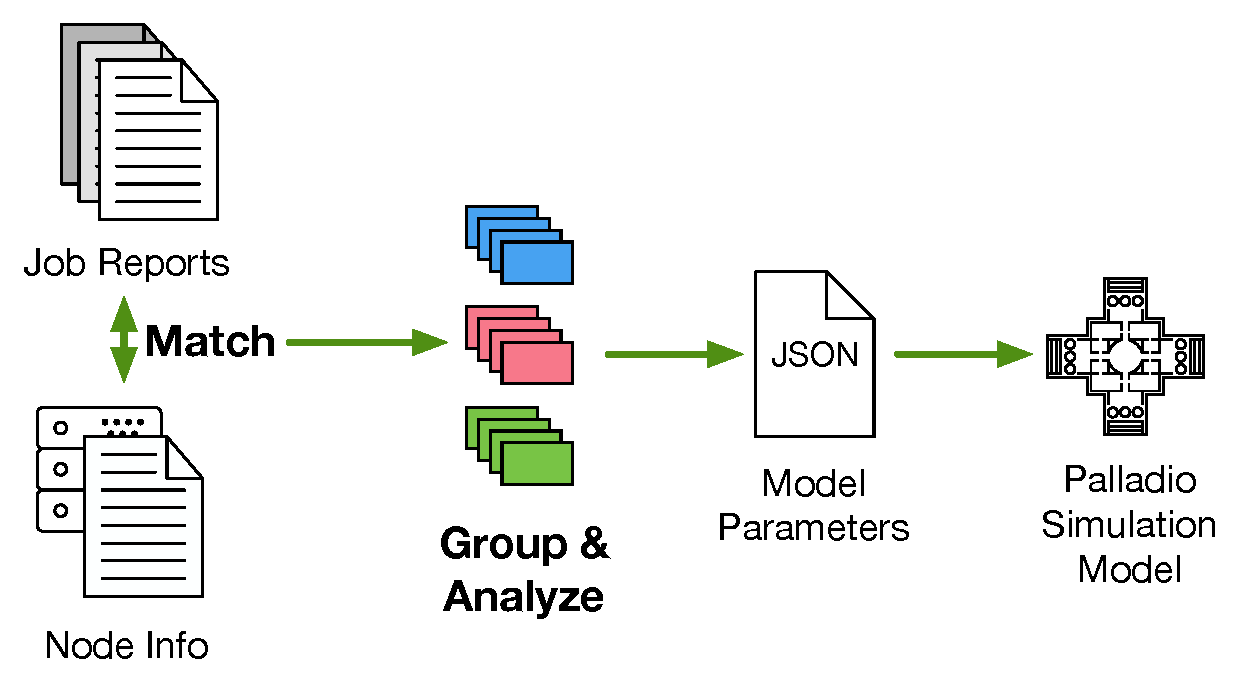
\includegraphics[width=0.45\linewidth]{images/process}
	\caption[]{The Simulation Process}
	\label{process}
\end{figure*}


\section{Modeling Computing Jobs and Resources}
\label{sec:model}
This section describes how the computing jobs and working nodes are modeled using Palladio.
The component model describes each type of CMS computing job, such as analysis or reprocessing jobs, with their resource demands. These demands are the \textit{CPU demand}, the\textit{ I/O demand}, the \textit{number of threads}, the \textit{required job slots}, and the \textit{number of demand rounds}.





\Cref{seff} shows the behaviour of the job during the simulation. After a job is scheduled on a resource container, it acquires the specified number of job slots or waits if the node has not sufficient free slots. Afterwards, the CPU and I/O demands of the job are processed. To avoid one big I/O operation at the start of a job and to make the simulated processing of I/O more continuous, it is modeled using iterations that reflect the number of processed events. Thus, for each iteration there are I/O and CPU resources needed. Rather than simulating each event, we simulate a fraction of the processed events, because the simulation of each event would harm the scalability of the simulation. 
While processing, the job uses the specified number of threads to process the CPU demand. After the job finished, it releases its acquired job slots. All of these parameters are specified as a probability function and are extracted from measured performance data as described in \Cref{sec:param}.


\begin{figure*}
	\centering
	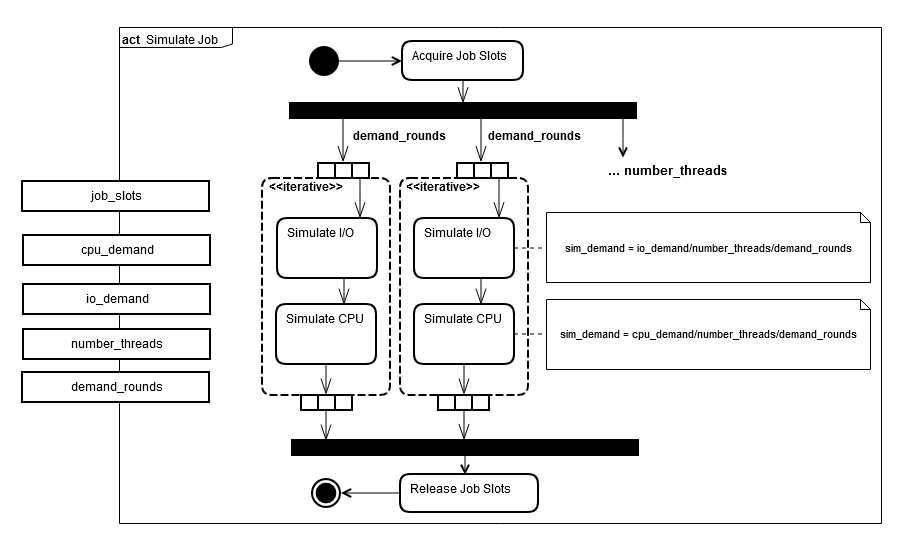
\includegraphics[width=0.82\linewidth]{images/seff}
	\caption[]{Model of Job Behavior}
	\label{seff}
\end{figure*}

Each type of working node in GridKa is modeled in the resource model. Each node type has a \textit{CPU and I/O processing rate}, \textit{number of cores}, \textit{number of job slots}, and \textit{number of instances} of this node type. The types of computing nodes are duplicated according to their specified number of instances as a preprocessing step of the simulation, resulting in the simulation of each working node.

At GridKa every type of computing job can run on every node, thus each job type is allocated on each computing node in the allocation model.

The usage model defines which and how many jobs are scheduled. To make sure that there is always a high load on the system, we used a closed workload with enough jobs that the system is fully utilized. Each job type has a configurable \textit{job share} of the overall load.

We extended Palladio with a \textit{load balancing strategy action}\footnote{https://github.com/PalladioSimulator/Palladio-Addon-ArchitecturalTemplates-LoadBalancing}, so that we can simulate load balancing strategies.
This load balancing strategy action is contained in a load balancing component.
In the assembly model all job components are connected with the load balancing component, which is the entry point of the system.
This action decides on which node a job should be scheduled based on the currently free job slots of each working node. The load balancing strategies can be extended to evaluate different strategies.



\section{Model Parameter Extraction and Model Creation}
\label{sec:param}

To obtain a comprehensive view both of the resource usage of CMS jobs executed at a WLCG grid site as well as the resources available there to process them, combining information from multiple data sources is required:
\begin{itemize}
    \item We acquire historical job monitoring information from several global CMS monitoring systems: Job reports from JobMonitoring and Workflow and Data Management framework job reports (FWJR documents) are archived on the \emph{analytix} Hadoop cluster.
    The latter are being archived on the cluster as part of the WMArchive project \cite{WMArchiveWorkloadArchive2018}.
    We collect job information using the \emph{CMSSpark} framework by Kuznetsov et al. \cite{cmsspark}.

    For this proof of concept, only jobs executed at the GridKa site were considered, but these data sources can be used to collect job reports from arbitrary WLCG sites.
    As these data sets contain different metrics for each executed job and not every job is contained in each data set, they are matched to each other to identify records that describe the same job execution prior to analysis.
    \item Site-specific performance data sets include the available nodes at the site and their performance information (including node benchmarks such as HS06 scores), which are available from local site monitoring systems.
    The simulation currently only includes computing jobs from CMS.
    As GridKa also processes jobs for other experiments, the number of available nodes at the site is scaled down to match the share of CMS workloads at the site in the time frame used for calibration.
    This share of resources is also collected from site-local monitoring information, as well as CPU efficiency reference data for the workloads executed in the same time frame.
\end{itemize}
To allow quick extraction of model parameters from these data sets, we implemented data set matching as well as the following analysis steps in an automated, configurable model parameter extraction tool written in Python.
Matching job information to local node performance information allows their resource usage to be decoupled from the hardware used to execute them, e.g. by combining the CPU time they used with node benchmarks of the machine they were executed on.

For the purposes of this proof of concept, jobs were then grouped according to their type as indicated in the job reports, but the extraction framework allows to be configured for arbitrary groupings of the extracted jobs.
Job resource requirement distributions for the different job types are extracted as distributions based on the empirical distributions in the data sets used for calibration, in the form of discrete probability density functions.

The parameter extraction tool\footnote{https://github.com/mxsg/CMS-Model-Calibration} exports model parameter sets as JSON files.
To simplify calibrating simulation models with these parameter sets, we created a Palladio plugin\footnote{https://github.com/mxsg/WLCG-Model-Construction} that can be used to automatically complete a blueprint of the simulation model (which defines the structure of the model as described in section \ref{sec:model}) with arbitrary parameter sets.
This ensures an efficient and flexible model creation process.

\section{Validation}
\label{validation}

\begin{figure}[h]
	\centering
	\vspace{-10px}
	\begin{subfigure}{0.48\linewidth}
		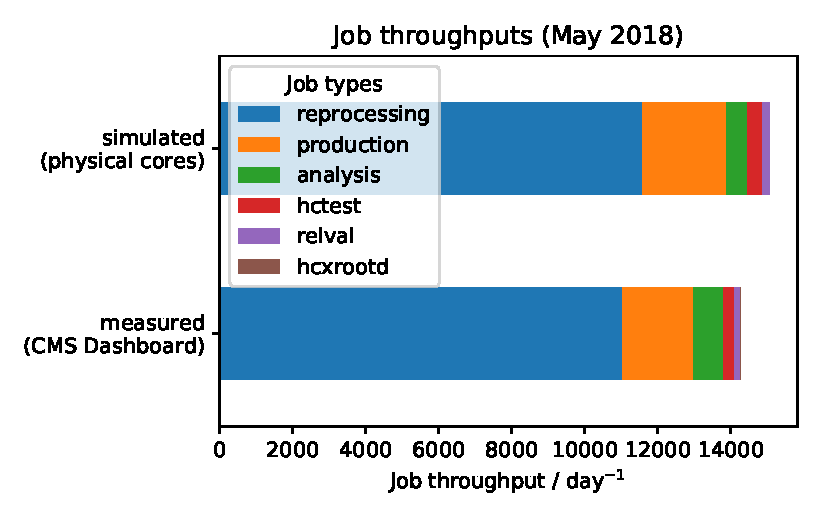
\includegraphics[width=\linewidth]{images/validation/throughputs}
	\end{subfigure}
	\begin{subfigure}{0.48\linewidth}
		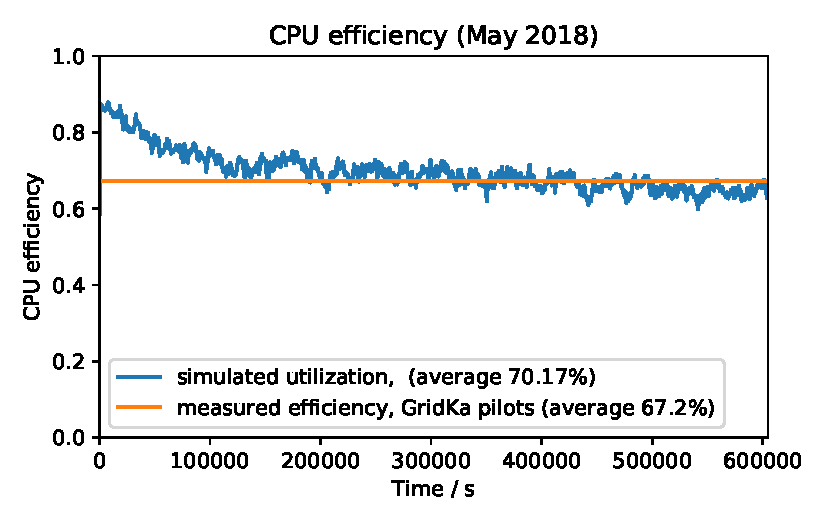
\includegraphics[width=\linewidth]{images/validation/utilizations}
	\end{subfigure}
	\vspace{-10px}
	\caption{Measured and simulated throughputs and CPU efficiency, job data from May 2018}
	\label{fig:validation}
\end{figure}
\vspace{10px}
\noindent To validate the model and simulation we simulated CMS jobs at GridKa in May 2018.
The job performance data was split into two equal sized calibration and test datasets by randomly sampling reports from the full data set.
For the validation we considered the following metrics: Overall throughput of jobs, shares of the job types, and the overall CPU efficiency of the site.
These metrics describe how well the simulation matches the measured performance data.
Comparisons between simulation results and measurements from the system are shown in \Cref{fig:validation}.
One result is that simulated throughput matches the reference with a difference of about 5.6\%.
Furthermore, the shares of the simulated and measured job types also match accurately.

The CPU utilization in the simulation and a comparison with the measured CPU efficiency are shown in \Cref{fig:validation}, which also makes the initial ramp-up of the simulation visible.
The overall average utilization in the simulation deviates from the reference by about 3\%, showing that even the current simplified model is capable of reproducing the metrics introduced above.
Additionally, the runtimes of the simulated jobs were measured: The average runtime of simulated jobs deviates by approximately 8\% from the measured runtimes in the test data set.

Simulating one week of CMS jobs at GridKa takes about 24 minutes on a laptop.
Thus, it is feasible to simulate several sites at once in a reasonable time, however simulating larger parts of the grid is future work.

\section{Related Work}
\label{related}
The MONARC project was started 1998 to help with the development of the initial design of the WLCG at CERN \cite{monarc2000models}.
However, after the initial design was developed, the project was discontinued in 2000 and thus no model and simulation of the WLCG was created. 
In 2004 a second version of the MONARC simulator was released with several improvements, such as simulation of data replication. However, MONARC2 showed scalability issues when simulating a Tier-2 site and accuracy issues regarding network load \cite{1742-6596-331-7-072038}.

There are a variety of grid and cloud simulators existing, of which SimGrid and CloudSim are two popular ones. 
However, both of them are implemented as libraries and not as standalone simulators. Thus, both are missing graphical model editors which makes the modeling of the computing jobs time-consuming \cite{simgrid,cloudsim}. The support of graphical editors is a big advantage of Palladio and increases its usability and efficiency. Another advantage of Palladio is the separation of the system into different models, which enables one to change on part of the system without modifying others. Furthermore, both do lack the support of an integrated visualization tool to display the results.  


CACTOS is an approach to cloud infrastructure automation and optimization \cite{cactos}.
One part of the approach is the CACTOS Runtime Toolkit for monitoring and resource management and another part is the CACTOS Prediction Toolkit for evaluation of alternative data center deployment scenarios and resource management algorithms. The Prediction Toolkit is built on Palladio and SimuLizar.
A first case studies in the context of chemical computing showed that the Prediction Toolkit has a high accuracy, but it was not tested on large systems yet \cite{rapidtesting}. However, due the required Runtime Toolkit CACTOS was not applicable in our use case.

Korenkov et. al simulated the JINR Tier1 site in 2016 \cite{jinr} and Hushchyn et al. created a simulation for the LHCb Grid in 2017 \cite{lhcb}. Both simulations focused on the effects of the location of the required job data on the throughput of the sites.
However, they neither modeled each working node nor modeled details of the scheduling process like job slots, thus both simulations would not be usable to simulate load balancing strategies on working node level.


\section{Outlook}
\label{outlook}
Our next steps are the evaluation of different design decisions. In this section a selection of possible design decisions that could be simulated are presented.

One possible design decision is a more sophisticated load balancing strategy that aims for a better resource utilization of the working nodes by scheduling a balanced share of CPU and I/O heavy jobs to it. To simulate this a new scheduling strategy must be implemented.

Another design decision would be to experiment with different sizes of pilot jobs, assuming that smaller pilot jobs result in a better utilization due less wasted CPU capacity in the draining phase of a pilot. For this use case the model must be extended with the explicit modeling of pilots jobs.

Additionally, the effects of integrating cloud resources could be simulated. The model must be extended with the cloud resources and the required network load to access the files from a site. Then a good load balancing strategy for the  integration of cloud resources could be evaluated, like only scheduling CPU heavy jobs to cloud resources and keeping I/O heavy jobs near the data.

Also the effects of data caches could be simulated. Firstly, several sites must be modeled to simulate their interactions. Secondly, the jobs must be parametrized with the possibility of remote access. Afterwards, the data cache with its hit rate should be modeled. Finally, the performance improvements of the data cache by transferring data from the cache and not from sites can be simulated.
\section{Conclusion}
\label{conlusion}

Computing resources for user analyses will become increasingly distributed and heterogeneous in the future and 
scheduling will be a key component for the efficient usage of the grid. We are confident that our approach helps to improve utilization of the grid and to be able to cope with the rising complexity of the system, thus serves the HEP community as a tool to solve the challenges created by the HL-LHC update.

We successfully simulated the CMS computing jobs at GridKa. To enable easy usage of the simulation we implemented an automated model parameter extraction and model creation. Furthermore, we extended Palladio to be able to simulate load balancing strategies. Our first results are promising and suggest that this approach can be used to simulate load balancing strategies accurately. Regarding scalability we are confident that several computing centers can be simulated in a sufficient time, however this is part of future work.

This proof of concept showed that an automated model parameter extraction and model creation is possible and that Palladio can be used to evaluate load balancing strategies for computing in HEP. In contrast to the existing simulations our simulation models a site in a more detailed way, enabling the evaluation of load balancing strategies on working node level. The next step is the evaluation of design decisions mentioned in \Cref{outlook}.




\bibliography{paper}

\end{document}



